\chapter{Design and implementation}\label{DesignAndImplementation}
\ifpdf
    \graphicspath{{Chapter3/Chapter3Figs/PNG/}{Chapter3/Chapter3Figs/PDF/}{Chapter3/Chapter3Figs/}}
\else
    \graphicspath{{Chapter3/Chapter3Figs/EPS/}{Chapter3/Chapter3Figs/}}
\fi

The aim of this chapter is to give a thorough description of our concrete implementation of the theoretical framework introduced
in Chapter \ref{TheoreticalFramework}. We list and provide an explanation of the individual
components and also explain our reasoning for certain design choices. In section \ref{WebApp} we present a proof-of-concept web application that 
we have developed in order to demonstrate how the different components can be integrated together to form a platform for event detection. 

\section{System Overview}
Figure \ref{SystemOverview} shows an overview of the system architecture which is a pipeline of the individual components we described
in Chapter \ref{TheoreticalFramework}. Each one of these components is depicted as an independent module in the figure.  
Initially, historical tweets from a service provider (Twitter API or another provider) are retrieved and stored in an 
appropriate format in the database. Subsequently, the system receives a stream of tweets from the database and processess and 
transforms them in a format that is appropriate for clustering. The next step in the pipeline is the actual clustering of the tweets 
in order to detect groups of tweets discussing the same topic. Then, the extracted clusters are processed in order to identify the events 
and generate their summaries. Finally, a visual representation of the results should be generated in order to aid understanding of the events.\\

\begin{figure}[htbp]
  \begin{center}
    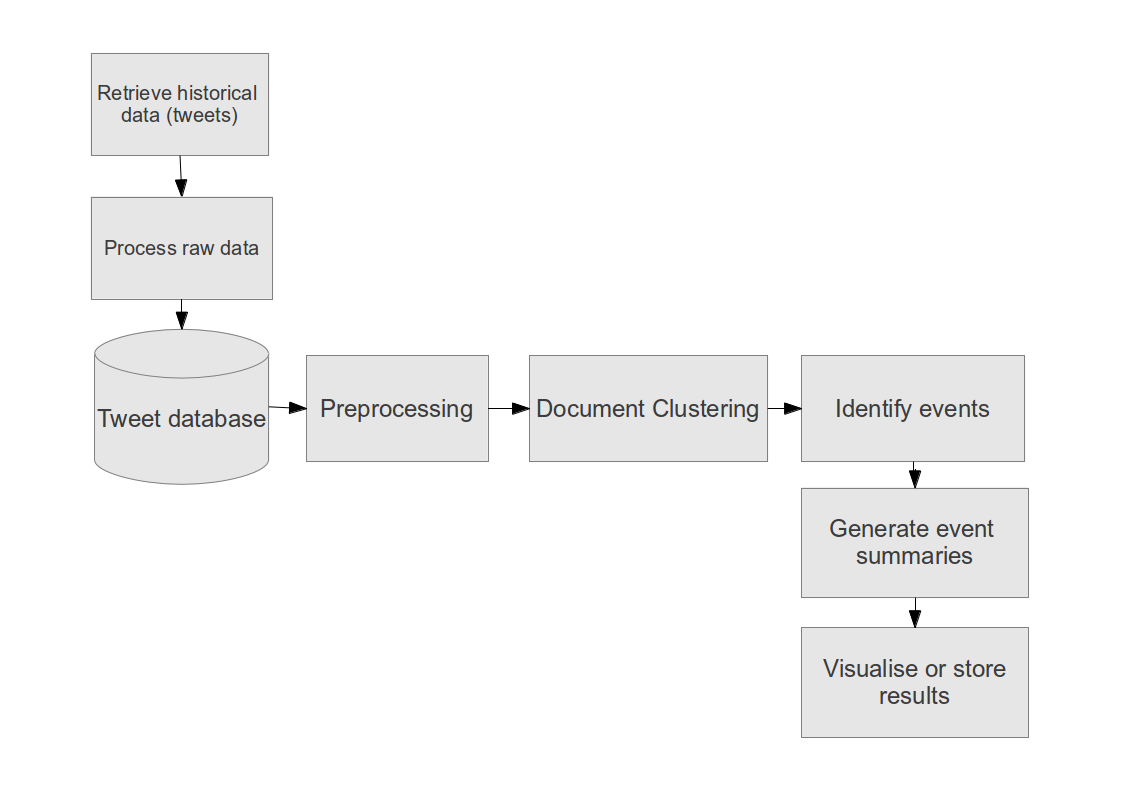
\includegraphics[height=3in, width=6in]{system-overview}
    \caption{System overview - The event extraction system comprises of several independent components.}
    \label{SystemOverview}
  \end{center}
\end{figure}

\subsection{Tools}
In the process of implementing the system we have mainly used our implementation of the algorithms but several third-party 
software libraries were used to implement the sub-components of the system. Here we describe the main tools we have used.\\ 

\begin{itemize}
 \item \textbf{Python:} 
 \item \textbf{Natural Language Toolkit (NLTK) :} 
 \item \textbf{Lucene:} 
 \item \textbf{Orange:} 
\end{itemize}\vspace{15pt}

\section{Data Retrieval}
A vital part of our system is the retrieval of a large amount of historical tweets. The first obvious choice is the Twitter API which provides tweets, user profiles and several metadata related to Twitter. They also provide a streaming API which is commonly used to collect tweets in real time. However, the main problem with the Twitter API is that it has a very restrictive limit policy (150 requests per hour) and it does not provide access to tweets posted more than a few days ago. This is a problem for our project since we require access to historical data. The solution is to use other archiving services and there are numerous possibilities. However, it is essential for us to have direct access to their database through an API and unfortunatelly, most of them do not provide an API. We have found that Topsy \footnote{http://topsy.com/} provides an excellent API \footnote{http://code.google.com/p/otterapi/} and direct access to tweets from 2009 up to the present day. Additionally, Topsy API is free and the limit policy allows us to retrieve our data easily. Therefore, we have decided to use Topsy Otter API with its Python bindings.

\section{Raw text processing}
The raw tweets received from Topsy are not processed and therefore we must apply some pre-processing steps before storing them in the database. The reasons for pre-processing were outlined clearly in Chapter \ref{TheoreticalFramework}. Figure \ref{RawTextProcessingOverview} depicts the sub-components of the raw text pre-processing module.\\

\begin{figure}[htbp]
  \begin{center}
    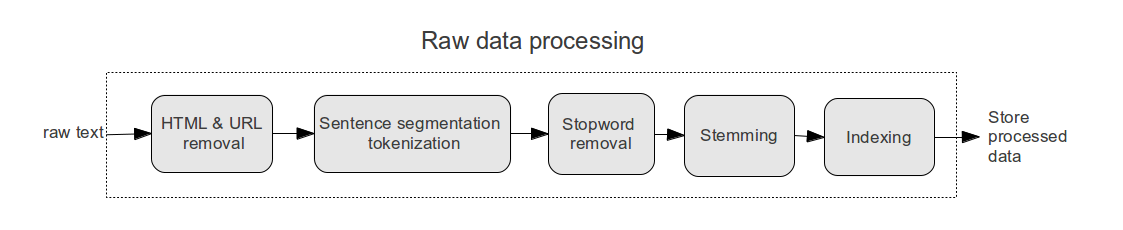
\includegraphics[height=1.5in, width=6in]{raw-data-processing}
    \caption{The raw data processing module - All the steps neccessary to convert raw documents to a format suitable for storage in a database.}
    \label{RawTextProcessingOverview}
  \end{center}
\end{figure} 

\textbf{HTML and URL removal:} Firstly, we need to clean the tweets from the URLs and HTML tags since they are useless for clustering. In order to do so we have used regular expressions which capture any possible format of URLs or HTML code.\\

\textbf{Sentence segmentation and tokenisation:} For the implementation of this module we have used the default sentence segmenter of NLTK and the WordPunctTokenizer to tokenise the resulting sentences. The reason we have used WordPunctTokenizer is due to the fact that it can handle alphabetic and non-alphabetic characters. Since it is common to use non-alphabetic characters in a tweet we could find an easy way to remove characters such as '.' and ','. Consider for example the following tweet:
 
\begin{figure}[htbp]
  \begin{center}
    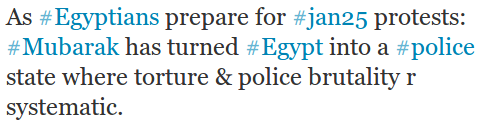
\includegraphics[height=1in, width=4in]{tweet-text}
    \label{TweetText}
  \end{center}
\end{figure}

The output from this module will be a list of words containing the terms \textbf{[ 'as', 'egyptians', 'prepare', 'for' 'jan25', 'protests', 'mumbarak', 'has', 'turned', 'egypt', 'into', 'a', 'police', 'state', 'where', 'torture', 'police', 'brutality', 'r', 'systematic' ]}. Note that characters '.', '\#', '\&' and ':' have been removed. \\

\textbf{Stopword removal:} The next step is to remove common English words that doesn't provide any information. NLTK provides a dictionary of the English stopwords and we have used it to filter out stopwords from the tweets. Using the list of words extracted for the example above the output of the stopword removal module will be: \textbf{['egyptians', 'prepare', 'jan25', 'protests', 'mumbarak', 'turned', 'egypt', 'police', 'state', 'torture', 'police', 'brutality', 'r', 'systematic' ]}

\textbf{Stemming:} Once we have the list of our terms we can use a stemming algorithm to reduce the words to their root. Our implementation uses the widely used Porter stemmer which is also implemented in NLTK. The final list of words after the stemming becomes \textbf{['egyptian', 'prepar', 'jan25', 'protest', 'mumbarak', 'turn', 'egypt', 'polic', 'state', 'tortur', 'polic', 'brutal', 'r', 'systemat' ]}\\

\textbf{Indexing:} Just before storing the tweets in the database we take a last step which is to index the tweets. For each word occuring in our corpus we aggregate all the tweets that contain that term and the position of that word in the document. Effectively, we create a mapping from a word to a list of documents. In our implementation the inverted index is very important since it allows us to construct term-documment vectors easily and filter terms and documents. For example, using our index we can find the words that appear either too often or less frequently and filter them out. This is used to reduce the dimensionality of our dataset by removing unneccesary words. Alternatively, we
can remove documents/tweets which contain keywords that appear too often or less frequently. In our implementation we have used PyLucene which is the Python equivalent of the Lucene indexing library. The library allow us to do what we have discussed above and in addition it provides helper functions such as the calculation of the TF-IDF weigtings for a dataset.
 
\section{Clustering}

So far we have managed to retrieve and store historical tweets in our database. The next module in our pipeline is to perform clustering on the tweets and identify clusters which discuss the same topic. The clustering module (Figure \ref{ClusteringOverview}) is responsible to construct the term-frequency vectors by processing the dataset and subsequently to apply a clustering algorithm on the dataset. 

\begin{figure}[htbp]
  \begin{center}
    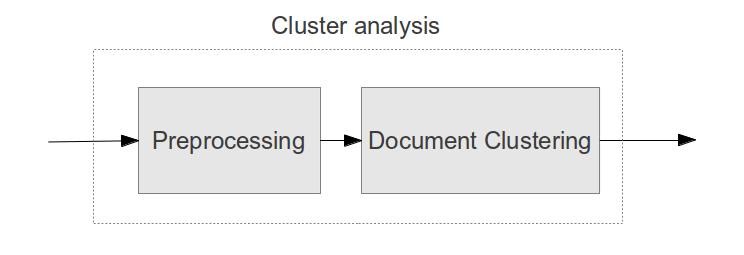
\includegraphics[height=1.5in, width=4in]{clustering-overview}
    \caption{The cluster analysis module - The dataset is processed to construct the term-frequency vectors and then a clustering algorithm is used to identify the clusters.}
    \label{ClusteringOverview}
  \end{center}
\end{figure} 

There are several candidates algorithms for clustering documents and we have decided to implement four of them. The theoretical background of these algorithms is outlined in Chapter \ref{TheoreticalFramework} and in Chapter \ref{Evaluation} we present a thorough comparison of these algorithms with respect to their performance in clustering tweets.  
In the next section we provide our implementation of these algorithms and the components that are needed for clustering. 

\subsection{AbstractClusterer and the derived clusterers}
The four different algorithms presented in this section are the k-Means, DBSCAN, non-negative matrix factorisation and online clusterers. Although these methods are fundamentally different they share some common functionality. For example the pre-processing steps, such as the construction of the term-frequency vectors is identical for all of them. Also, all of the algorithms output the clusters using the same format and therefore the methods for visualising the clusters will be identical. The architecture of the software components responsible for implementing the clustering functionality tries to incorporate this common functionality as well as accomodating the different core implementation of each algorithm. The UML diagram (Figure \ref{UMLClusterers}) below illustrates the different components of the clustering module. The AbstractClusterer class implements all the common functionalities such as add\_document, construct\_term\_freq\_matrix, plot\_scatter and dump\_clusters\_to\_file. Since each algorithm uses a different method to perform the actual clustering task, the AbstractClusterer class do not provide any implementation for the "run" function. This is the responsibility of each derived clusterer. 

\begin{figure}[htbp]
  \begin{center}
    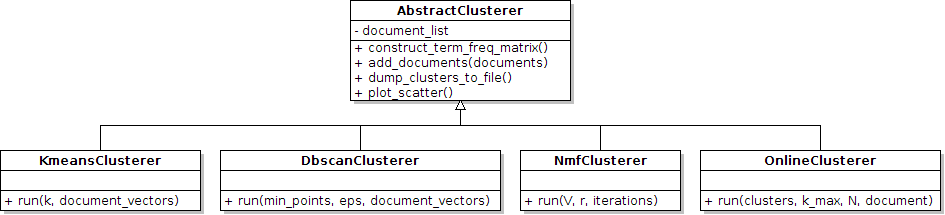
\includegraphics[height=2.0in, width=6in]{clusterers-uml}
    \caption{The four derived clusterers share common functionality which is implemented in the AbstractClusterer class. }
    \label{UMLClusterers}
  \end{center}
\end{figure}    
 
The main functionality of the AbstractClusterer is to construct the term-frequency vector for each document and consequently the term-frequency matrix $a$ which has a row for each document and a column for each distinct term in the dataset. This will convert the corpus in the vector space representation. Listing \ref{AbstractClustererSnippet} shows the pseudocode for implementing the construct\_term\_freq\_matrix function. We retrieve the dataset from the database and we find all the distinct terms that occur across all the documents. Then the term-frequency matrix is initialised and we iterate over the documents filling in the elements of the matrix with the TF-IDF weight of each term. The function returns the matrix $a$.

\begin{lstlisting}[language=Python, label=AbstractClustererSnippet, caption=Pseudocode for constructing the term-frequency matrix for a dataset]
def construct_term_freq_matrix(corpus):
  '''
  Inputs: 
  corpus: The collections of documents we will cluster
  
  Outputs:
  a: A nxm matrix where n is the number of documents 
     in the corpus and m the number of distinct terms
     in the corpus.  
  '''
  terms = find_distinct_terms(corpus)
  a = initialise_term_frequency_matrix(rows=len(corpus), 
                                        columns=len(terms))
  
  for i, document in enumerate(corpus):
    for term in document
      a[i][term] = tf_idf(term, document, corpus)
    
  return a 
\end{lstlisting}

In the next pages we discuss the implementation of the concrete clusterers and we show some preliminary results of the clustering process.\\

\textbf{k-Means:} Listing \ref{KmeansClustererSnippet} shows the pseudocode for k-Means clustering algorithm. The algorithm works by randomly initialising k centroids and then finding out which document vectors are closest to the centroid. Then the centroid is recomputed based on the mean of the vectors belonging to this centroid and this mean value becomes the new centroid. An additional check is performed again to ensure that all the vectors are still belonging to that cluster after the recomputation of the centroid. This procedure is repeated until there are previous cluster membership has not changed. Note that the distance() function can be any of the three distance measures described in the previous chapter.

\begin{lstlisting}[language=Python, label=KmeansClustererSnippet, caption=Pseudocode for k-Means algorithm]
def run(k, document_vectors):
  '''
  Inputs: 
  k: the number of clusters
  document_vectots: the set of n document 
                     vectors I={i1,i2,..,in}
  
  Outputs:
  C: cluster centroids {c1, c2, ..., ck}
  m: I --> C the cluster membership
  '''
  C = random_centroid_initialisation()
  
  distances = []
  for vector in document_vectors
    for c in C:
      dist = distance(c, vector)
      distances.append(dist)
    m[vector] = min(distances)

  while has_changed(m):
    for c in C:
      c = recompute_centroid(c, vectors_of(c))   
    
    for vector in document_vectors
      for c in C:
        dist = distance(c, vector)  
        distances.append(dist)
      m[vector] = min(distances)
  return C, m

\end{lstlisting}
\vspace{10 mm}
\textbf{DBSCAN:} Listing \ref{DbscanClustererSnippet} shows the pseudocode for the DBSCAN clustering algorithm. Initially,
all documents are marked as unvistied and the cluster list is empty. Then the algorithm randomly selects a new document vector, marks it
as visited and finds all its neighbors than are within a distance eps. The set of neighbors is called ε-neighborhood and we denote it here by N. In order to calculate the distance we use one of the three predefined distance measures. If N does not contain at least min\_pts then we mark this vector as a noise point. Otherwise, a new cluster is created which contains this vector and all the objects in N are added to a candidate set. DBSCAN iteratively adds to the new cluster those documents in the N that do not belong to any cluster. For any object in the ε-neighborhood DBSCSAN checks again its own ε-neighborhood N' and if it has at least min\_pts those document vectors are added to the N. This continues, with DBSCAN adding new documents in the new cluster, until N is empty. Finally, to find the next cluster DBSCAN selects a new unvisited document vector and continues the same process until all vectors have been visited.  

\begin{lstlisting}[language=Python, label=DbscanClustererSnippet, caption=Pseudocode for DBSCAN algorithm]
def run(min_points, eps, document_vectors):
  '''
  Inputs: 
  eps: the radius parameter
  min_pts: the neighborhood density threshold.
  document_vectors: the set of n document vectors 
                     I={i1,i2,..,in}
  
  Outputs:
  C: the clusters and the document vectors 
     belonging to them
  '''
  C = [] #The cluster list
  mark_all_vectors_as_unvisited(document_vectors)
  
  while not all_is_visited(document_vectors):  
    vector = pick_random(document_vectors)
    mark_as_visited(vector)
    neighbors = get_neighbors(document_vectors, vector)
    if len(neighbors) >= eps:
      new_cluster = create_cluster(vector) 
      C.append(new_cluster)
      for n_vector in neighbors:
        if not is_visited(n_vector) 
          mark_as_visited(n_vector)
          n_neighbors=get_neighbors(document_vectors,n_vector)
          if len(n_neighbors) >= eps:
            neighbors.append(n_neighbors)
        if not_in_cluster(n_vector):
          new_cluster.add(n_vector)
    else:
      mark_as_noise(vector) 
  return C
\end{lstlisting}
\vspace{10 mm}
\textbf{Non-negative matrix factorisation:} Our implementation is based for NMF is based on the paper [put ref here for Learning the parts of objects by nonnegative matrix factorization]. The method accepts as input the term-frequency matrix $V$ the number of basis vectors to generate $r$ and the number of optimisation iterations. The algorithm starts from non-negative initialisations for W and H and then iteratively updates W and H until a factorisation $V \approx WH$ such that $| V - WH |$ is minimal. If the number of maximum iterations has not been reached and the error did not change since the last iteration then the algorithm halts and return W and H. Listing \ref{NMFClustererSnippet} shows the pseudocode for the NMF algorithm. The notation $A.T$ indicates that we shoud take the transpose of the matrix $A$.
  
\begin{lstlisting}[language=Python, label=NmfClustererSnippet, caption=Pseudocode for the NMF algorithm]
def run(V, r, iterations):
  '''
  Inputs: 
  V: the matrix to factorize
  r: number of basis vectors to generate
  iterations: number of optimisation
             iterations to perform
  
  Outputs:
  W: a set of r basis vectors
  H: represenations of the columns of V in 
     the basis given by W
  '''
  
  C = size(V,1) #dimensionality of examples (# rows)
  N = size(V,2) #number of examples (columns)

  W = rand(N,r);
  H = rand(r,C);
  
  previous_error = 0
  error = 0
  for i in xrange(iterations):

    #Update W
    W2 = dot(dot(W, H), H.T) + 10**-9
    W *= dot(V[:,:], H.T)
    W /= W2
    
    #Update H
    H2 = dot(dot(W.T, W), H) + 10**-9
    H *= dot(W.T, V[:,:])
    H /= H2                                     
    
    previous_error = error
    error = sqrt( sum((V[:,:] - dot(W, H))**2 ))
    
    if i > 1 and error:
      if previous_error == error:
        break
  return W, H
  
\end{lstlisting}

\textbf{Online:} 

\section{Identifying events}

\section{Generating automatic summaries}

\section{Classifying users}

\section{Optimisations}

\section{Developing a proof-of-concept web application}\label{WebApp}

\section{Summary}

% ------------------------------------------------------------------------


%%% Local Variables: 
%%% mode: latex
%%% TeX-master: "../thesis"
%%% End: 
